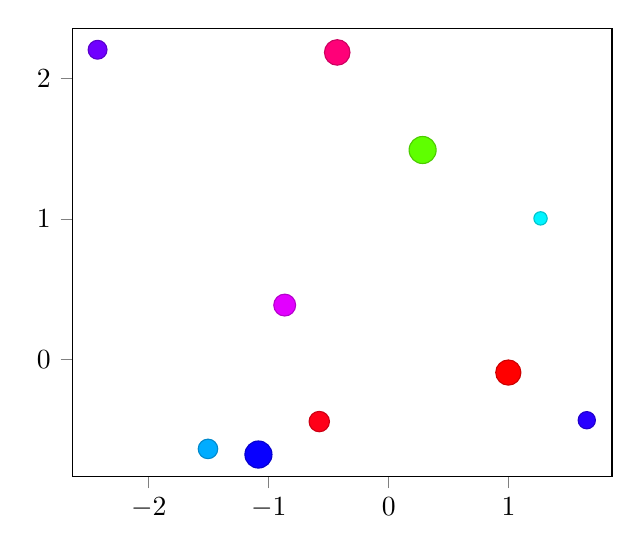
\begin{tikzpicture}

\begin{axis}[
tick align=outside,
tick pos=left,
x grid style={white!69.01960784313725!black},
xmin=-2.63725258881175, xmax=1.86149632855493,
y grid style={white!69.01960784313725!black},
ymin=-0.835853216474104, ymax=2.35933144192702
]
\addplot [only marks, scatter, scatter src=explicit, colormap={mymap}{[1pt]
  rgb(0pt)=(1,0,0);
  rgb(10pt)=(1,0.9375,0);
  rgb(11pt)=(0.96875,1,0);
  rgb(21pt)=(0.03125,1,0);
  rgb(22pt)=(0,1,0.0625);
  rgb(32pt)=(0,1,1);
  rgb(42pt)=(0,0.0625,1);
  rgb(43pt)=(0.03125,0,1);
  rgb(53pt)=(0.96875,0,1);
  rgb(54pt)=(1,0,0.9375);
  rgb(63pt)=(1,0,0.09375)
}, visualization depends on={\thisrow{sizedata} \as\perpointmarksize}, scatter/@pre marker code/.append style={/tikz/mark size=\perpointmarksize}]
table [x=x, y=y, meta=colordata]{%
x                      y                      colordata              sizedata
-1.08563060330056 -0.678886151622054 -0.255619370530597 4.89256733647935
0.997345446583586 -0.0947089689368911 -2.79858910546072 4.54836597410367
0.282978498051992 1.49138962612429 -1.77153310450985 4.88667343302704
-1.50629471391809 -0.638901996684651 -0.699877234597917 3.52635650804
-0.578600251968536 -0.443981959646065 0.927462431758582 3.68070378912419
1.65143653709715 -0.434351275618517 -0.173635682790216 3.1180697130645
-2.42667924339307 2.20593008272546 0.00284591589681102 3.40549357402605
-0.428912628856177 2.18678608897379 0.688222711102285 4.61077361155706
1.26593625870553 1.00405389787888 -0.879536343009052 2.41282221214437
-0.866740402265102 0.386186399174856 0.283627323807291 3.95066098824534
};
\end{axis}

\end{tikzpicture}